\documentclass{beamer}
\usetheme[style=beta]{epyt}
\usepackage{macros_beamer}
\usepackage{caption}
\usepackage{subcaption}
\usepackage[portuguese]{babel}
\title{Solução numérica da equação da onda unidimensional}
\subtitle{Modo fundamental}
\date{02 de julho de 2026}
\author{Leonardo Suarez}
\institute{Instituto de Matemática e Estatística - UFRGS}

\usepackage[backend=biber, style=ieee]{biblatex}\addbibresource{referencias_numerico.bib}
\setbeamertemplate{bibliography item}{\insertbiblabel}

\begin{document}

\nocite{burden, IK, moyses_ondas, stencil}

\begin{frame}
    \titlepage
\end{frame}

\section{o problema físico}

\begin{frame}
    Consideramos a \alert{equação da onda unidimensional}
    \begin{equation}
        u_{tt} = u_{xx}, \quad 0 < x < 1, \quad t > 0
    \end{equation} com condições de contorno e iniciais
    \begin{align}
        u(0, t) &= 0, \quad u(1, t) = 0, \quad t > 0 \\
        u(x, 0) &= \sin(\pi x), \quad u_t(x, 0) = 0, \quad 0 < x < 1.
    \end{align} A solução analítica é dada por
    \begin{align}
        u(x, t) &= \sin(\pi x) \cos(\pi t)
    \end{align}

    \begin{figure}
        \centering
        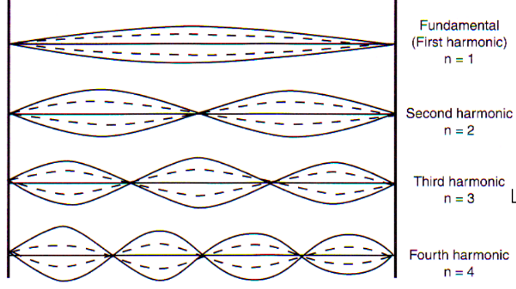
\includegraphics[width=0.6\textwidth, keepaspectratio]{harmonics.png}
        \label{fig:harmonics}
    \end{figure}
\end{frame}

\section{discretização da edp}

\begin{frame}{método explícito de diferenças finitas}
    Aproximamos as derivadas por \alert{diferenças finitas centrais}, obtendo a equação a diferenças
    \begin{equation}\label{eq:solucao_diferencas_finitas}
        w_{i, j+1} = 2(1 - \lambda^2) w_{i, j} + \lambda^2 (w_{i+1, j} + w_{i-1, j}) - w_{i, j-1},
    \end{equation} para \(i = 1, 2, \ldots, m-1\) e \(j = 1, 2, \ldots, N-1\).
    \begin{figure}
        \centering
        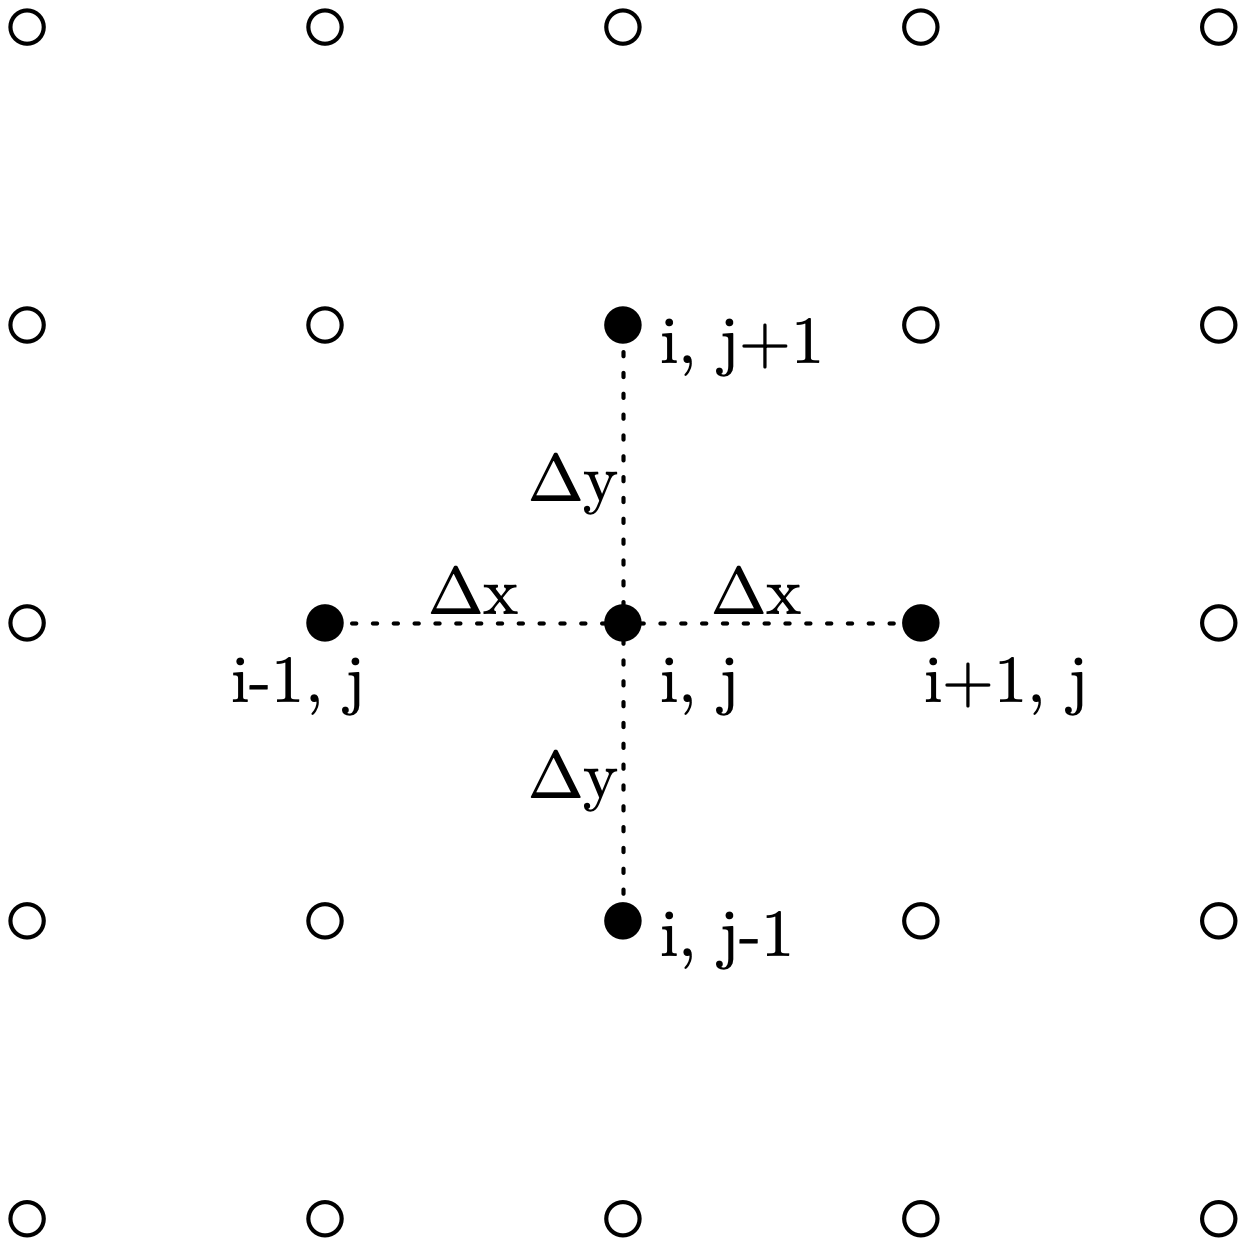
\includegraphics[width=0.4\textwidth, keepaspectratio]{five-point-stencil.png}
    \end{figure}
\end{frame}

\begin{frame}
    Para computar \(w_{i, t_1}\), aproximamos \(u(x_i, t_1)\) por um polinômio de Maclaurin de segunda ordem em \(t\) e usamos a condição inicial \(u_t(x, 0) = 0\). Ainda, aproximamos \(\frac{\partial^2}{\partial x^2}\sin(\pi x_i)\) por diferenças centrais, obtendo
    \begin{equation}
        w_{i, 1} = (1 - \lambda^2) w_{i, 0} + \frac{\lambda^2}{2} (w_{i+1, 0} + w_{i-1, 0}),
    \end{equation} para \(i = 1, 2, \ldots, m-1\).
\end{frame}

\section{resultados}

\begin{frame}{\(\lambda = 1\)}
    \begin{figure}[H]
        \centering
        \begin{subfigure}{0.48\textwidth}
            \centering
            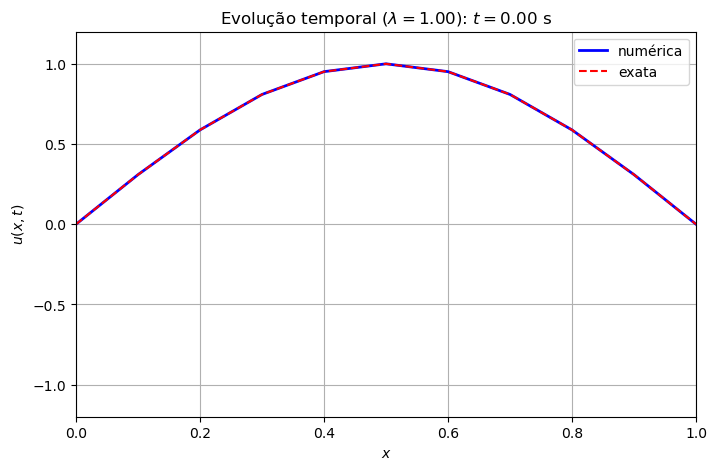
\includegraphics[width=\textwidth]{wave_1_t_0.00.png}
            \label{fig:wave_1_t000}
        \end{subfigure}
        \hfill
        \begin{subfigure}{0.48\textwidth}
            \centering
            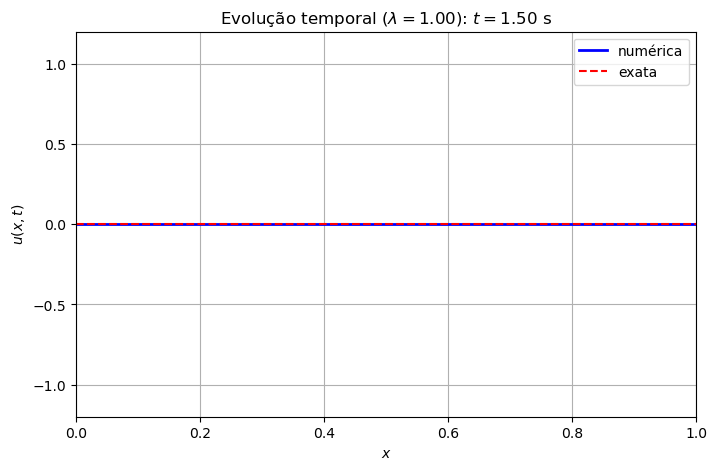
\includegraphics[width=\textwidth]{wave_1_t_1.50.png}
            \label{fig:wave_1_t150}
        \end{subfigure}
                
        \begin{subfigure}{0.48\textwidth}
            \centering
            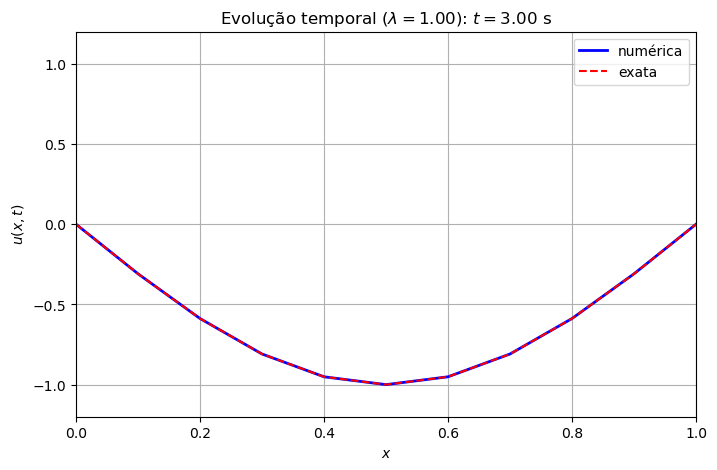
\includegraphics[width=\textwidth]{wave_1_t_3.00.png}
            \label{fig:wave_1_t300}
        \end{subfigure}
        \hfill
        \begin{subfigure}{0.48\textwidth}
            \centering
            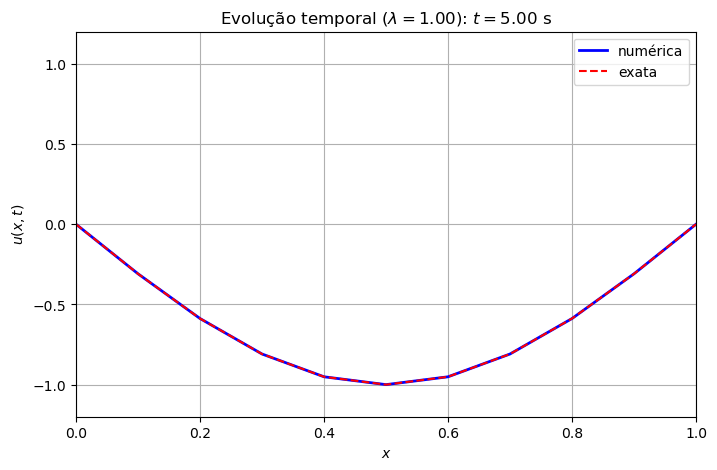
\includegraphics[width=\textwidth]{wave_1_t_5.00.png}
            \label{fig:wave_1_t500}
        \end{subfigure}        
        \label{fig:wave_1}
    \end{figure}
\end{frame}

\begin{frame}{\(\lambda = 0.2\)}
    \begin{figure}[H]
        \centering
        \begin{subfigure}{0.48\textwidth}
            \centering
            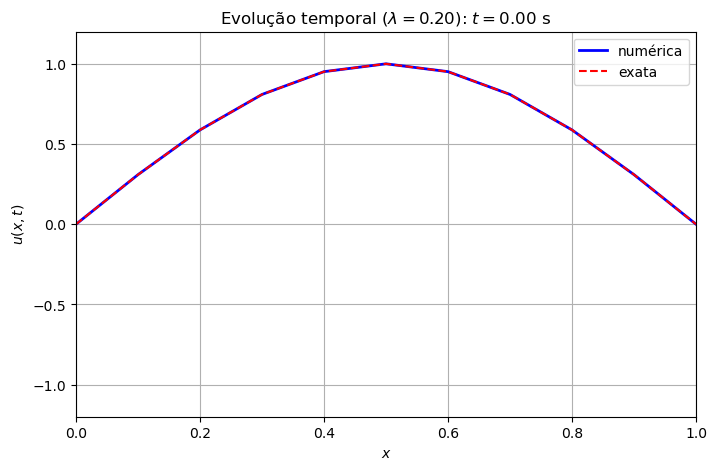
\includegraphics[width=\textwidth]{wave_2_t_0.00.png}
            \label{fig:wave_2_t000}
        \end{subfigure}
        \hfill
        \begin{subfigure}{0.48\textwidth}
            \centering
            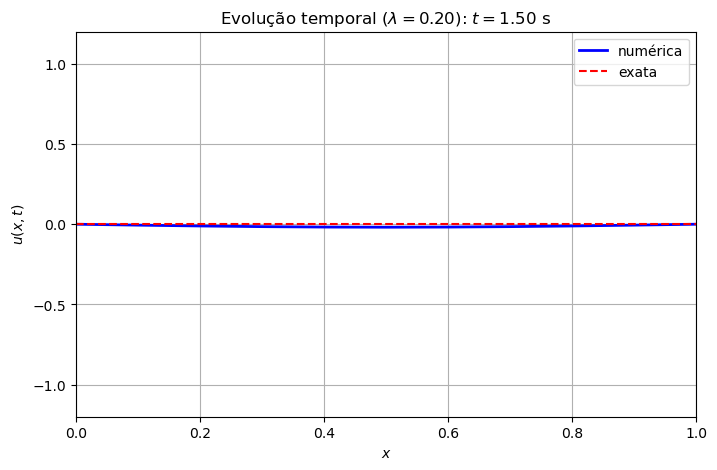
\includegraphics[width=\textwidth]{wave_2_t_1.50.png}
            \label{fig:wave_2_t150}
        \end{subfigure}
        \begin{subfigure}{0.48\textwidth}
            \centering
            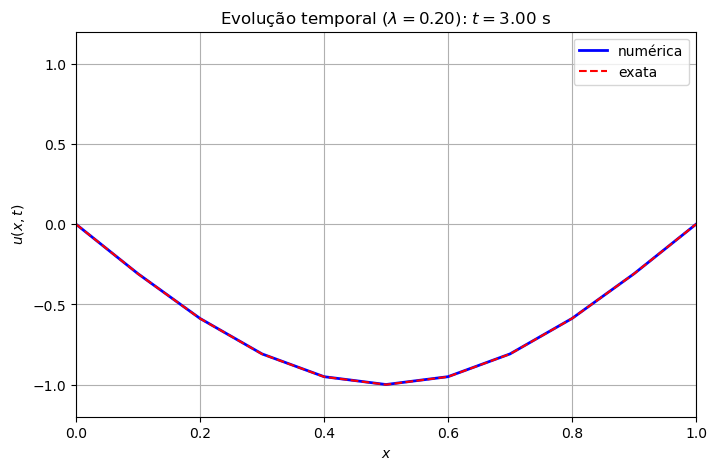
\includegraphics[width=\textwidth]{wave_2_t_3.00.png}
            \label{fig:wave_2_t300}
        \end{subfigure}
        \hfill
        \begin{subfigure}{0.48\textwidth}
            \centering
            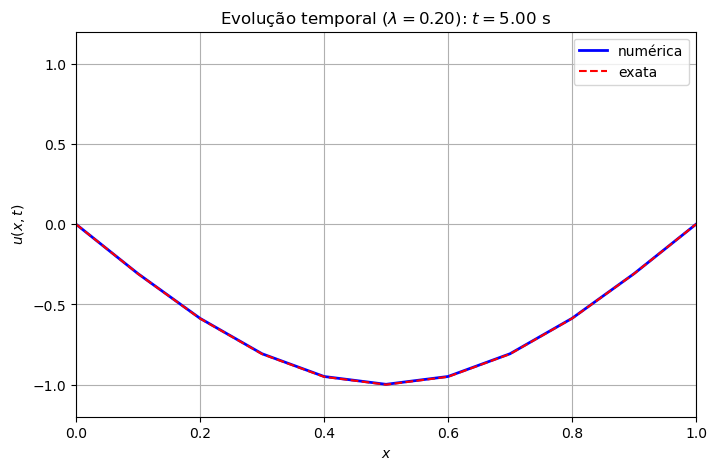
\includegraphics[width=\textwidth]{wave_2_t_5.00.png}
            \label{fig:wave_2_t500}
        \end{subfigure}
        \label{fig:wave_2}
    \end{figure}
\end{frame}

\begin{frame}{\(\lambda = 1.2\)}
    \begin{figure}[H]
        \centering
        \begin{subfigure}{0.48\textwidth}
            \centering
            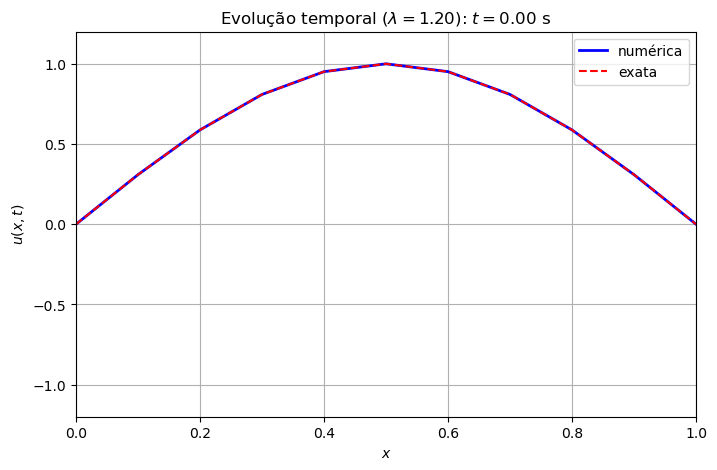
\includegraphics[width=\textwidth]{wave_3_t_0.00.png}
            \label{fig:wave_3_t000}
        \end{subfigure}
        \hfill
        \begin{subfigure}{0.48\textwidth}
            \centering
            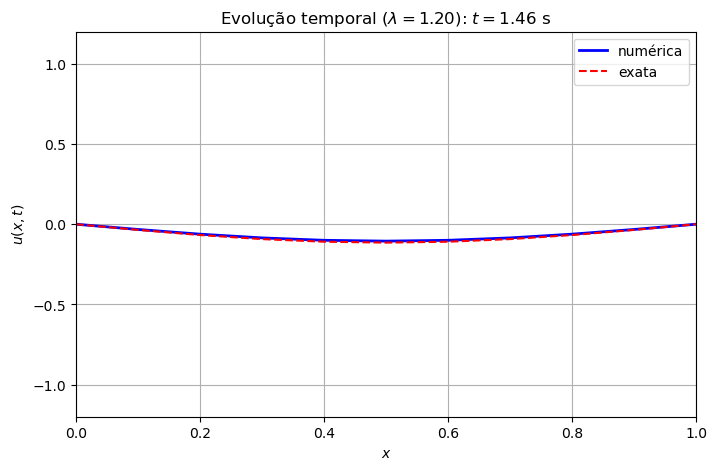
\includegraphics[width=\textwidth]{wave_3_t_1.46.png}
            \label{fig:wave_3_t146}
        \end{subfigure}
        
        \begin{subfigure}{0.48\textwidth}
            \centering
            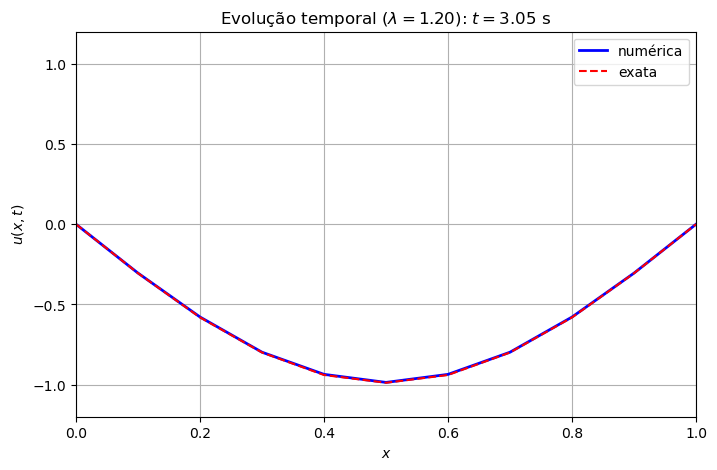
\includegraphics[width=\textwidth]{wave_3_t_3.05.png}
            \label{fig:wave_3_t305}
        \end{subfigure}
        \hfill
        \begin{subfigure}{0.48\textwidth}
            \centering
            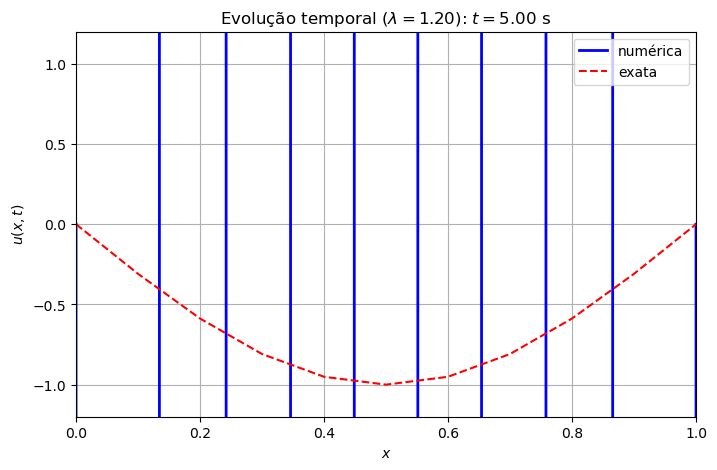
\includegraphics[width=\textwidth]{wave_3_t_5.00.png}
            \label{fig:wave_3_t500}
        \end{subfigure}
        \label{fig:wave_3}
    \end{figure}
\end{frame}

\section{análise do erro e de estabilidade}

\begin{frame}{condição necessária de estabilidade}
    O método explícito de difernças finitas é estável se a \alert{condição de Courant-Friedrichs-Lewy (CFL)} for satisfeita, ou seja, se \(\lambda = k/h \leq 1\)\cite[489]{IK}.
\end{frame}

\begin{frame}{\(\lambda = 1\)}
    \begin{itemize}
        \item o método é estável;
        \item a solução numérica coincide com a solução analítica.
    \end{itemize}
    \begin{table}[H]
        \centering
        \label{tab:resultados_lambda_1}
        \begin{tabular}{cccc}
            \toprule
            \(x_i\) & \(w_{i, 5}\) & \(u(x_i, 5)\) & \(|w_{i, 5} - u(x_i, 5)|\) \\
            \midrule
            0.0 & 0.00000000 & -0.00000000 & 0.0000e+00 \\
            0.1 & -0.30901699 & -0.30901699 & 5.5511e-17 \\
            0.2 & -0.58778525 & -0.58778525 & 1.1102e-16 \\
            0.3 & -0.80901699 & -0.80901699 & 0.0000e+00 \\
            0.4 & -0.95105652 & -0.95105652 & 5.5511e-16 \\
            0.5 & -1.00000000 & -1.00000000 & 0.0000e+00 \\
            0.6 & -0.95105652 & -0.95105652 & 4.4409e-16 \\
            0.7 & -0.80901699 & -0.80901699 & 0.0000e+00 \\
            0.8 & -0.58778525 & -0.58778525 & 5.5511e-16 \\
            0.9 & -0.30901699 & -0.30901699 & 5.5511e-17 \\
            \bottomrule
        \end{tabular}
    \end{table}
\end{frame}

\begin{frame}{\(\lambda = 0.2\)}
    \begin{itemize}
        \item o método é estável;
        \item o erro numérico coincide com o erro de truncamento \(\mathcal{O}(k^2 + h^2)\).
    \end{itemize}
    \begin{table}[H]
        \centering
        \label{tab:resultados_lambda_0.2}
        \begin{tabular}{cccc}
            \toprule
            \(x_i\) & \(w_{i, 5}\) & \(u(x_i, 5)\) & \(|w_{i, 5} - u(x_i, 5)|\) \\
            \midrule
            0.0 & 0.00000000 & -0.00000000 & 0.0000e+00 \\
            0.1 & -0.30842395 & -0.30901699 & 5.9304e-04 \\
            0.2 & -0.58665722 & -0.58778525 & 1.1280e-03 \\
            0.3 & -0.80746439 & -0.80901699 & 1.5526e-03 \\
            0.4 & -0.94923132 & -0.95105652 & 1.8252e-03 \\
            0.5 & -0.99808088 & -1.00000000 & 1.9191e-03 \\
            0.6 & -0.94923132 & -0.95105652 & 1.8252e-03 \\
            0.7 & -0.80746439 & -0.80901699 & 1.5526e-03 \\
            0.8 & -0.58665722 & -0.58778525 & 1.1280e-03 \\
            0.9 & -0.30842395 & -0.30901699 & 5.9304e-04 \\
            \bottomrule
        \end{tabular}
    \end{table}
\end{frame}

\begin{frame}{\(\lambda = 1.2\)}
    \begin{itemize}
        \item o método não é estável;
        \item o erro numérico explode e se afasta da solução analítica.
    \end{itemize}
    \begin{table}[H]
        \centering
        \label{tab:resultados_lambda_1.2}
        \begin{tabular}{cccc}
            \toprule
            \(x_i\) & \(w_{i, 5}\) & \(u(x_i, 5)\) & \(|w_{i, 5} - u(x_i, 5)|\) \\
            \midrule
            0.0 & 0.00000000 & -0.00000000 & 0.0000e+00 \\
            0.1 & -173015.37874265 & -0.30901699 & 1.7302e+05 \\
            0.2 & 328811.25437226 & -0.58778525 & 3.2881e+05 \\
            0.3 & -451966.12936866 & -0.80901699 & 4.5197e+05 \\
            0.4 & 530419.43046658 & -0.95105652 & 5.3042e+05 \\
            0.5 & -556672.80998304 & -1.00000000 & 5.5667e+05 \\
            0.6 & 528431.36623167 & -0.95105652 & 5.2843e+05 \\
            0.7 & -448749.37386477 & -0.80901699 & 4.4875e+05 \\
            0.8 & 325594.49886836 & -0.58778525 & 3.2560e+05 \\
            0.9 & -171027.31450774 & -0.30901699 & 1.7103e+05 \\
            \bottomrule
        \end{tabular}
    \end{table}
\end{frame}

\section*{referências}

\begin{frame}{referências}
    \printbibliography
\end{frame}

\end{document}